\FloatBarrier
\subsection{Results}
The figures generated by the Python code visually confirm the controller's effectiveness and match their counterparts in the paper.

\subsubsection{Figure 1: System Output vs. Reference Signal}
 This plot is the most direct measure of success. The system output ($y$, solid line) is shown to converge rapidly to the sinusoidal reference signal ($y_d$, dashed line). After a brief initial transient period, the tracking error becomes very small, demonstrating that the primary control objective has been met. This result visually matches Figure 1 in the paper, confirming the controller's high-precision tracking performance.
\begin{figure}[H]
	\centering
	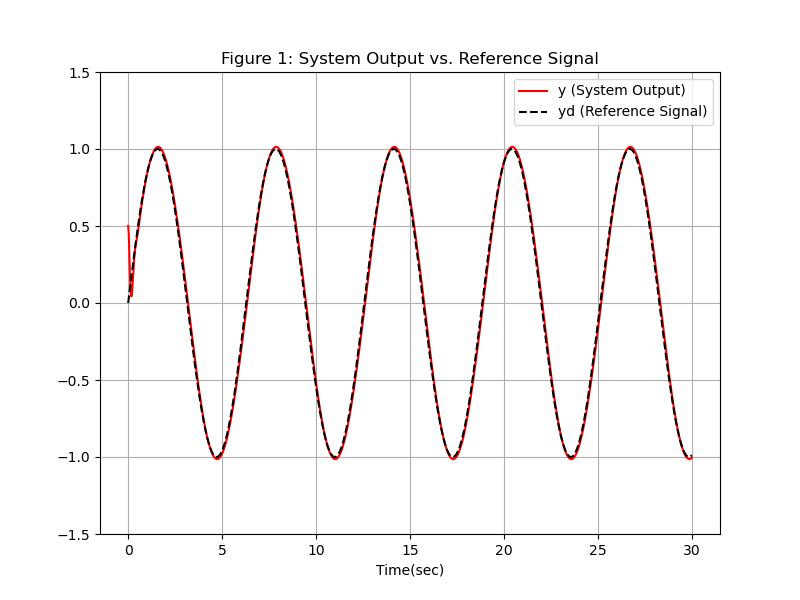
\includegraphics[width=0.7\textwidth]{images/sim1.png}
	\caption{System Output vs. Reference Signal}
	\label{fig:fig41}
\end{figure}

\clearpage
\subsubsection{Figure 2: State Variable $z_2$} 
The stability analysis guarantees that all signals in the closed-loop system remain bounded. This plot shows the trajectory of the internal state $z_2$. As predicted by the theory, the state oscillates but remains well within a finite bound, never diverging to infinity. This provides visual evidence of the internal stability of the system and matches the behavior shown in Figure 2 of the paper.
\begin{figure}
	\centering
	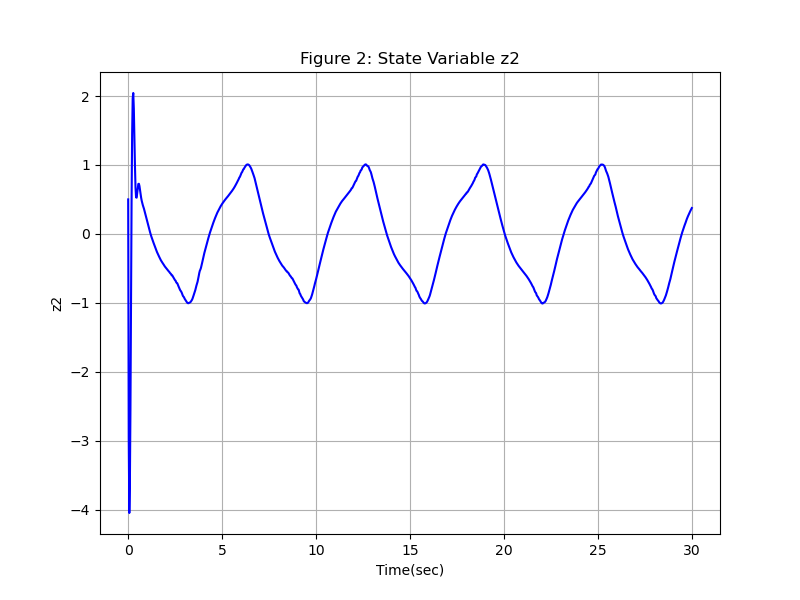
\includegraphics[width=0.7\textwidth]{images/sim2.png}
	\caption{State Variable $z_2$}
	\label{fig:fig42}
\end{figure}

\clearpage
\subsubsection{Figure 3: Adaptive Parameters}
 This figure displays the time evolution of the adaptive fuzzy logic parameters, $\theta_1$ and $\theta_2$. Starting from their initial conditions of zero, both parameters converge smoothly to stable, constant values. This is a critical result, as it signifies that the adaptive laws are working correctly and the fuzzy systems have successfully "learned" the necessary information to approximate and counteract the unknown nonlinearities within the plant. This behavior is identical to that shown in Figure 3 in the paper.
\begin{figure}
	\centering
	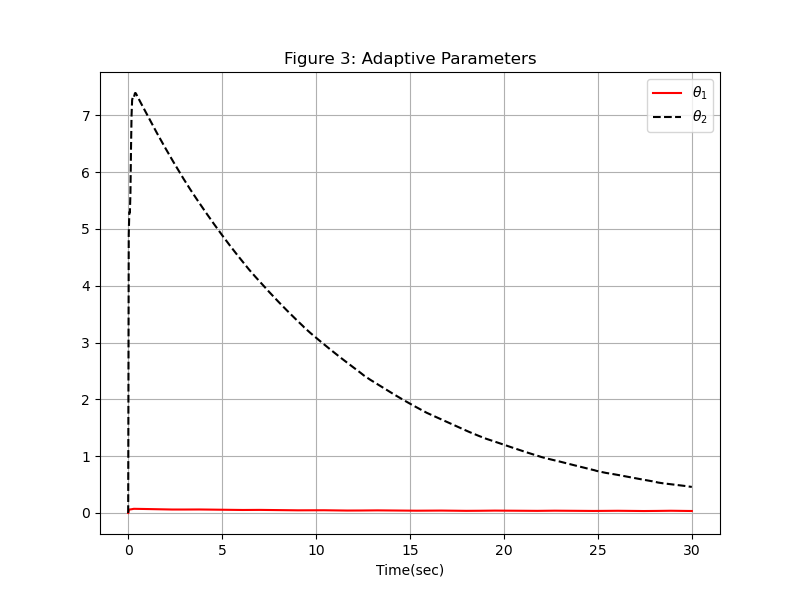
\includegraphics[width=0.7\textwidth]{images/sim3.png}
	\caption{Adaptive Parameters}
	\label{fig:fig43}
\end{figure}

\clearpage
\subsubsection{Figure 4: Quantizer Output}
 This plot reveals the nature of the actual control signal being fed to the system. Instead of a smooth curve, it is a step-like signal that jumps between discrete levels. This confirms the correct implementation of the hysteretic quantizer and, more importantly, demonstrates the controller's robustness. The system maintains excellent tracking performance even when driven by this non-ideal, quantized input, validating the design's practicality for digital systems and matching the results of Figure 4 in the paper.
\begin{figure}
	\centering
	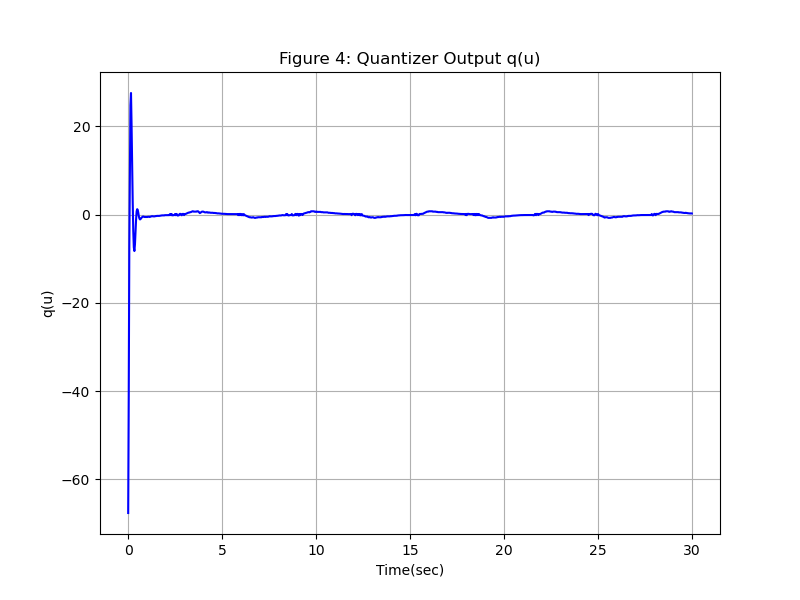
\includegraphics[width=0.7\textwidth]{images/sim4.png}
	\caption{Quantizer Output}
	\label{fig:fig44}
\end{figure}



 
